\documentclass[10pt,a4paper]{article}
\usepackage[margin=16mm]{geometry}
\usepackage[T1]{fontenc}
\usepackage{helvet,graphicx,xcolor}
\renewcommand{\familydefault}{\sfdefault}
\pagestyle{empty}
\newcommand{\classification}{RESEARCH DEMONSTRATION | NOT FOR OPERATIONAL USE}
\begin{document}
\begin{center}\color{red}\small\textbf{\classification}\end{center}
{\LARGE\textbf{Antarctic Fast Ice Watch}}\par
\medskip
Davis | 2021-10-24\par
\medskip
\textbf{PRIMARY PRODUCT | FAST-ICE EXTENT AND CHANGE}\par
\medskip
SYNTHETIC TEST DATA. This bulletin tests the software and layout; it describes no observed Davis conditions.\par
\begin{center}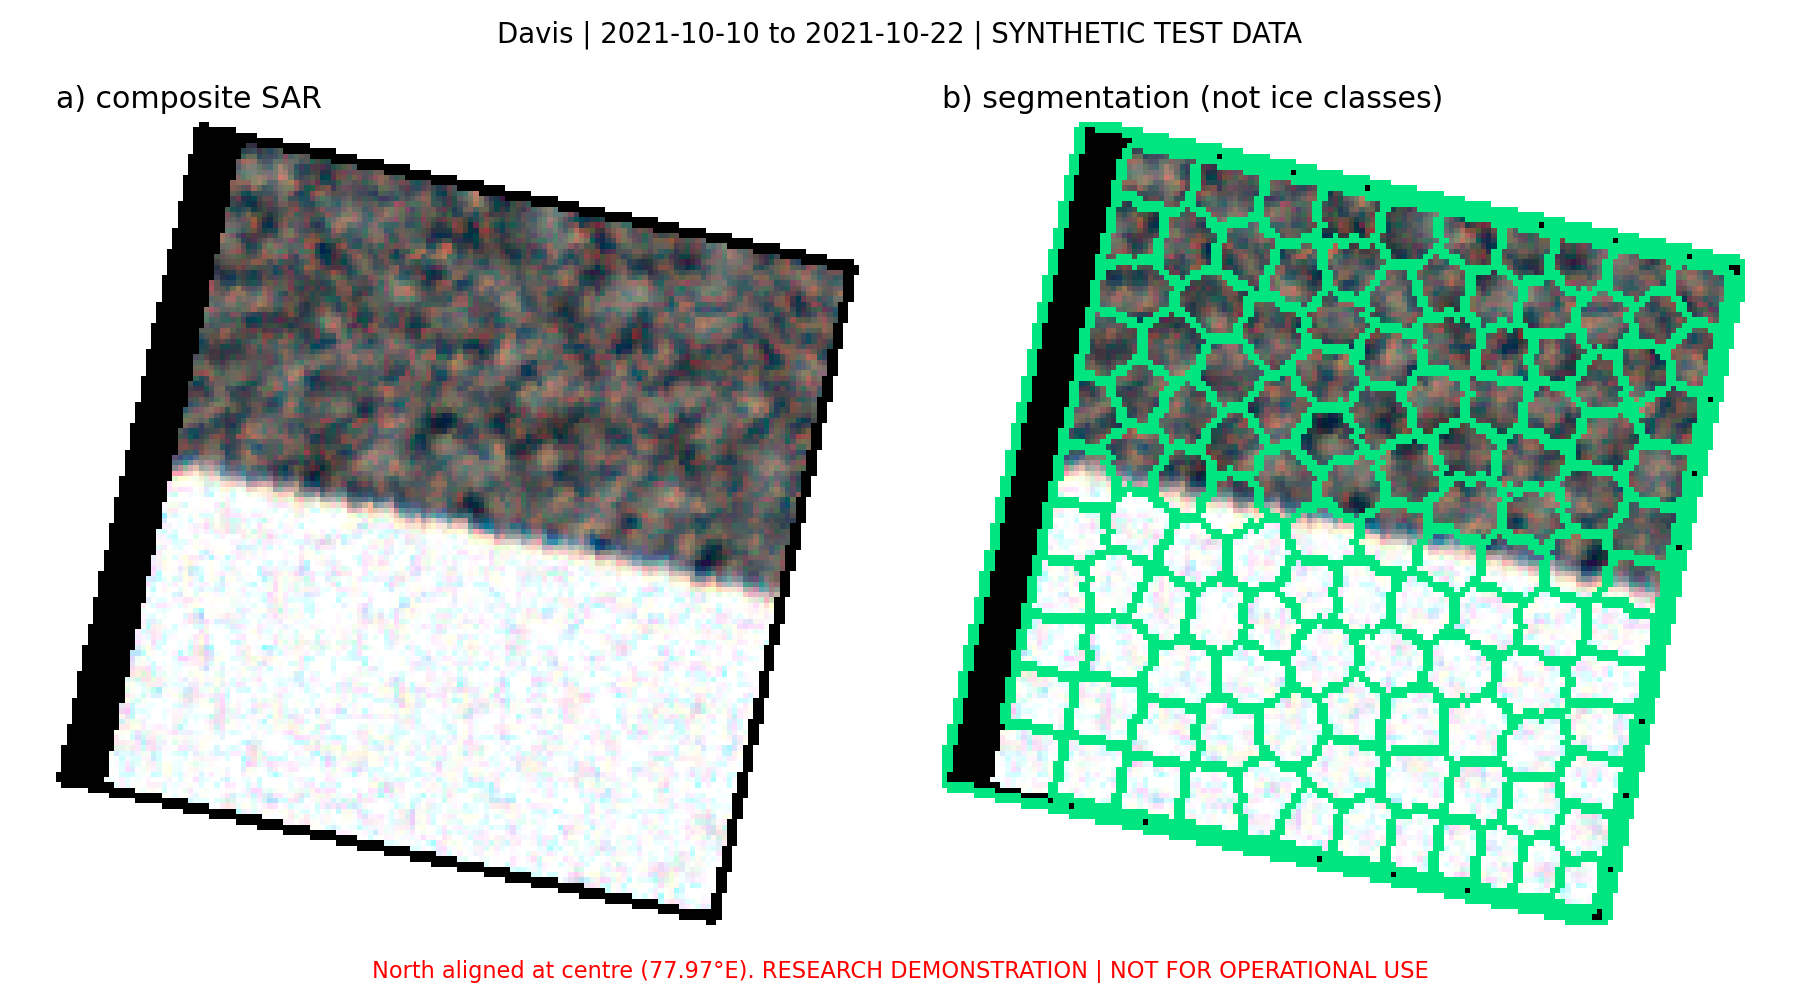
\includegraphics[width=\linewidth,height=95mm,keepaspectratio]{primary.png}\end{center}
\textbf{Coverage and quality}\par
Segmentation pixel spacing: 200 × 200 m; valid texture fraction 88.5\%. Acquisition baseline: 12.0 days.\par
\medskip
No reviewed land/ice-shelf mask supplied. Segmentation includes unmasked surfaces. Not validated for operational use SLIC differs from the supplied SAM research workflow\par
\medskip
\textbf{ADDITIONAL PRODUCT | SWOT FREEBOARD}\par
Not yet processed in this primary-product milestone. No SWOT observations or freeboard values are represented here.\par
\vfill
\begin{center}\color{red}\small\textbf{\classification}\end{center}
\end{document}
